% Options for packages loaded elsewhere
\PassOptionsToPackage{unicode}{hyperref}
\PassOptionsToPackage{hyphens}{url}
%
\documentclass[
]{article}
\usepackage{amsmath,amssymb}
\usepackage{lmodern}
\usepackage{iftex}
\ifPDFTeX
  \usepackage[T1]{fontenc}
  \usepackage[utf8]{inputenc}
  \usepackage{textcomp} % provide euro and other symbols
\else % if luatex or xetex
  \usepackage{unicode-math}
  \defaultfontfeatures{Scale=MatchLowercase}
  \defaultfontfeatures[\rmfamily]{Ligatures=TeX,Scale=1}
\fi
% Use upquote if available, for straight quotes in verbatim environments
\IfFileExists{upquote.sty}{\usepackage{upquote}}{}
\IfFileExists{microtype.sty}{% use microtype if available
  \usepackage[]{microtype}
  \UseMicrotypeSet[protrusion]{basicmath} % disable protrusion for tt fonts
}{}
\makeatletter
\@ifundefined{KOMAClassName}{% if non-KOMA class
  \IfFileExists{parskip.sty}{%
    \usepackage{parskip}
  }{% else
    \setlength{\parindent}{0pt}
    \setlength{\parskip}{6pt plus 2pt minus 1pt}}
}{% if KOMA class
  \KOMAoptions{parskip=half}}
\makeatother
\usepackage{xcolor}
\usepackage[margin=1in]{geometry}
\usepackage{color}
\usepackage{fancyvrb}
\newcommand{\VerbBar}{|}
\newcommand{\VERB}{\Verb[commandchars=\\\{\}]}
\DefineVerbatimEnvironment{Highlighting}{Verbatim}{commandchars=\\\{\}}
% Add ',fontsize=\small' for more characters per line
\usepackage{framed}
\definecolor{shadecolor}{RGB}{248,248,248}
\newenvironment{Shaded}{\begin{snugshade}}{\end{snugshade}}
\newcommand{\AlertTok}[1]{\textcolor[rgb]{0.94,0.16,0.16}{#1}}
\newcommand{\AnnotationTok}[1]{\textcolor[rgb]{0.56,0.35,0.01}{\textbf{\textit{#1}}}}
\newcommand{\AttributeTok}[1]{\textcolor[rgb]{0.77,0.63,0.00}{#1}}
\newcommand{\BaseNTok}[1]{\textcolor[rgb]{0.00,0.00,0.81}{#1}}
\newcommand{\BuiltInTok}[1]{#1}
\newcommand{\CharTok}[1]{\textcolor[rgb]{0.31,0.60,0.02}{#1}}
\newcommand{\CommentTok}[1]{\textcolor[rgb]{0.56,0.35,0.01}{\textit{#1}}}
\newcommand{\CommentVarTok}[1]{\textcolor[rgb]{0.56,0.35,0.01}{\textbf{\textit{#1}}}}
\newcommand{\ConstantTok}[1]{\textcolor[rgb]{0.00,0.00,0.00}{#1}}
\newcommand{\ControlFlowTok}[1]{\textcolor[rgb]{0.13,0.29,0.53}{\textbf{#1}}}
\newcommand{\DataTypeTok}[1]{\textcolor[rgb]{0.13,0.29,0.53}{#1}}
\newcommand{\DecValTok}[1]{\textcolor[rgb]{0.00,0.00,0.81}{#1}}
\newcommand{\DocumentationTok}[1]{\textcolor[rgb]{0.56,0.35,0.01}{\textbf{\textit{#1}}}}
\newcommand{\ErrorTok}[1]{\textcolor[rgb]{0.64,0.00,0.00}{\textbf{#1}}}
\newcommand{\ExtensionTok}[1]{#1}
\newcommand{\FloatTok}[1]{\textcolor[rgb]{0.00,0.00,0.81}{#1}}
\newcommand{\FunctionTok}[1]{\textcolor[rgb]{0.00,0.00,0.00}{#1}}
\newcommand{\ImportTok}[1]{#1}
\newcommand{\InformationTok}[1]{\textcolor[rgb]{0.56,0.35,0.01}{\textbf{\textit{#1}}}}
\newcommand{\KeywordTok}[1]{\textcolor[rgb]{0.13,0.29,0.53}{\textbf{#1}}}
\newcommand{\NormalTok}[1]{#1}
\newcommand{\OperatorTok}[1]{\textcolor[rgb]{0.81,0.36,0.00}{\textbf{#1}}}
\newcommand{\OtherTok}[1]{\textcolor[rgb]{0.56,0.35,0.01}{#1}}
\newcommand{\PreprocessorTok}[1]{\textcolor[rgb]{0.56,0.35,0.01}{\textit{#1}}}
\newcommand{\RegionMarkerTok}[1]{#1}
\newcommand{\SpecialCharTok}[1]{\textcolor[rgb]{0.00,0.00,0.00}{#1}}
\newcommand{\SpecialStringTok}[1]{\textcolor[rgb]{0.31,0.60,0.02}{#1}}
\newcommand{\StringTok}[1]{\textcolor[rgb]{0.31,0.60,0.02}{#1}}
\newcommand{\VariableTok}[1]{\textcolor[rgb]{0.00,0.00,0.00}{#1}}
\newcommand{\VerbatimStringTok}[1]{\textcolor[rgb]{0.31,0.60,0.02}{#1}}
\newcommand{\WarningTok}[1]{\textcolor[rgb]{0.56,0.35,0.01}{\textbf{\textit{#1}}}}
\usepackage{graphicx}
\makeatletter
\def\maxwidth{\ifdim\Gin@nat@width>\linewidth\linewidth\else\Gin@nat@width\fi}
\def\maxheight{\ifdim\Gin@nat@height>\textheight\textheight\else\Gin@nat@height\fi}
\makeatother
% Scale images if necessary, so that they will not overflow the page
% margins by default, and it is still possible to overwrite the defaults
% using explicit options in \includegraphics[width, height, ...]{}
\setkeys{Gin}{width=\maxwidth,height=\maxheight,keepaspectratio}
% Set default figure placement to htbp
\makeatletter
\def\fps@figure{htbp}
\makeatother
\setlength{\emergencystretch}{3em} % prevent overfull lines
\providecommand{\tightlist}{%
  \setlength{\itemsep}{0pt}\setlength{\parskip}{0pt}}
\setcounter{secnumdepth}{-\maxdimen} % remove section numbering
\ifLuaTeX
  \usepackage{selnolig}  % disable illegal ligatures
\fi
\IfFileExists{bookmark.sty}{\usepackage{bookmark}}{\usepackage{hyperref}}
\IfFileExists{xurl.sty}{\usepackage{xurl}}{} % add URL line breaks if available
\urlstyle{same} % disable monospaced font for URLs
\hypersetup{
  pdftitle={SG\_LB\_BMEG591E\_FinalProject},
  hidelinks,
  pdfcreator={LaTeX via pandoc}}

\title{SG\_LB\_BMEG591E\_FinalProject}
\author{}
\date{\vspace{-2.5em}2023-04-05}

\begin{document}
\maketitle

Introduction:

Our analysis is based on the paper published by Ha et al.~(2023)
entitled: ``Reduced expression of alanyl aminopeptidase is a robust
biomarker of non-familial adenomatous polyposis and non-hereditary
nonpolyposis colorectal cancer syndrome early-onset colorectal cancer''
(\url{https://doi.org/10.1002/cam4.5675}). The authors have made their
sequencing data (fastqs) and read counts file publicly available on the
GEO datbase:
\url{https://www.ncbi.nlm.nih.gov/geo/query/acc.cgi?acc=GSE213092}. We
chose this analysis because it involved many concepts that we covered in
class, but also went beyond these and required learning some new
techniques. Cancer biomarker discovery is a research interest of Liam's
lab, so this paper is relevant to potential projects he may carry out
down the road.

This study aimed to identify differential gene expression markers to
distinguish early-onset colorectal cancer from late-onset colorectal
cancer of the subtypes non-familial adenomatous polyposis and
non-hereditary nonpolyposis.The group performed RNA-seq of 49
early-onset and 50 late-onset colorectal cancer samples. They analyzed
differentially-expressed genes between these groups and filtered them
based on log2FC, logCPM, and P-values. They validated the identified
differentially-expressed genes using data from TCGA (The Cancer Genome
Atlas) database, based on similar expression profiles. Based on this
validation, they identified the gene analyl aminopeptidase (ANPEP) as
significantly downregulated in early-onset colorectal cancer patients in
both their cohort and the TCGA cohort. This association was further
supported by methylation data and information from the GTEx and
GSE196006 datasets. The study concluded that the gene ANPEP was
significantly down-regulated in early-onset colorectal cancer, and could
serve as a novel biomarker.

The scope of our analysis is to carry out the methods described in
section 2.2: Bulk RNA sequencing and data analysis. In these steps, the
authors used the fastq files output from RNAseq to obtain normalized
read counts, and used these to produce the heatmap shown in Figure 1A
and the volcano plot shown in Figure 2B. These steps were used to
identify genes that had significant differential expression between the
early-onset and late-onset groups in the 99 patient samples. These steps
precede the comparison with TCGA data that ultimately led the authors to
single out ANPEP as a novel biomarker.

Methods and Results:

Part I: Pre-processing fastqs to obtain read counts

To demonstrate the pre-processing steps for generating a read counts
file from fastq files as performed by the authors, we use only 4 fastq
files, two from the early-onset group and two from the late-onset group.
As there are 99 samples with 2 fastq files each in the whole dataset,
the analysis would be too time-consuming if we used all the available
files.

The files are named as follows:

LateOnset\_SRR21523090\_pass\_1.fastq.gz
LateOnset\_SRR21523090\_pass\_2.fastq.gz

LateOnset\_SRR21523091\_pass\_1.fastq.gz
LateOnset\_SRR21523091\_pass\_2.fastq.gz

EarlyOnset\_SRR21523117\_pass\_1.fastq.gz
EarlyOnset\_SRR21523117\_pass\_2.fastq.gz

EarlyOnset\_SRR21523118\_pass\_1.fastq.gz
EarlyOnset\_SRR21523118\_pass\_2.fastq.gz

In the following script, we tried to carry out all pre-processing steps
only for the sample EarlyOnset\_SRR21523117. We then incorporated all of
these steps into a pipeline that could be used to process any number of
samples.

\begin{enumerate}
\def\labelenumi{\arabic{enumi}.}
\tightlist
\item
  Check quality of raw fastqs using fastqc
\end{enumerate}

\begin{Shaded}
\begin{Highlighting}[]

\VariableTok{sample}\OperatorTok{=}\NormalTok{EarlyOnset\_SRR21523117}
\ExtensionTok{fastqc} \AttributeTok{{-}o}\NormalTok{ ./fastQC\_output }\VariableTok{$sample}\StringTok{"\_pass\_1.fastq.gz"} \VariableTok{$sample}\StringTok{"\_\_pass\_2.fastq.gz"}
\end{Highlighting}
\end{Shaded}

As shown below, the fastq file failed the per base sequence content and
adapter content quality metrics. This showed that we needed to trim
adapters and indexes.

\begin{figure}
\centering
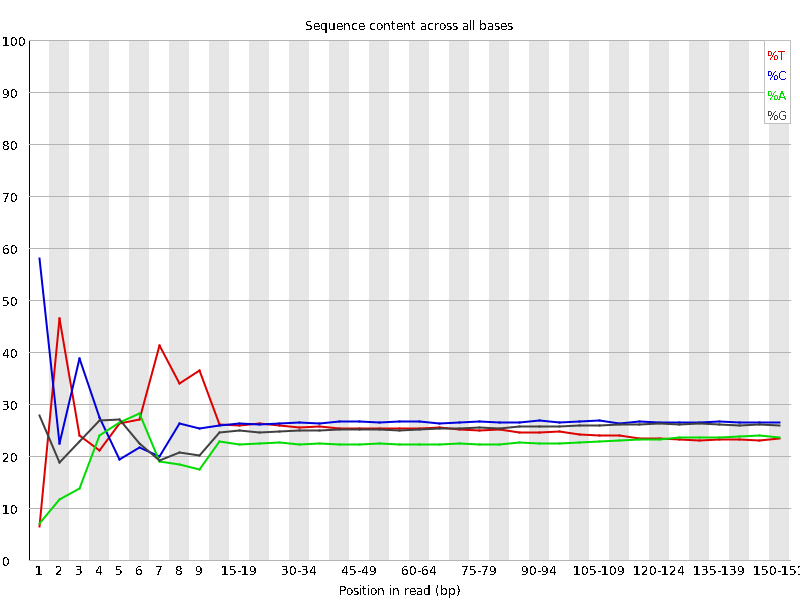
\includegraphics{./EarlyOnset_SRR21523117_pass_1_fastqc_basecontent.png}
\caption{sequence content}
\end{figure}

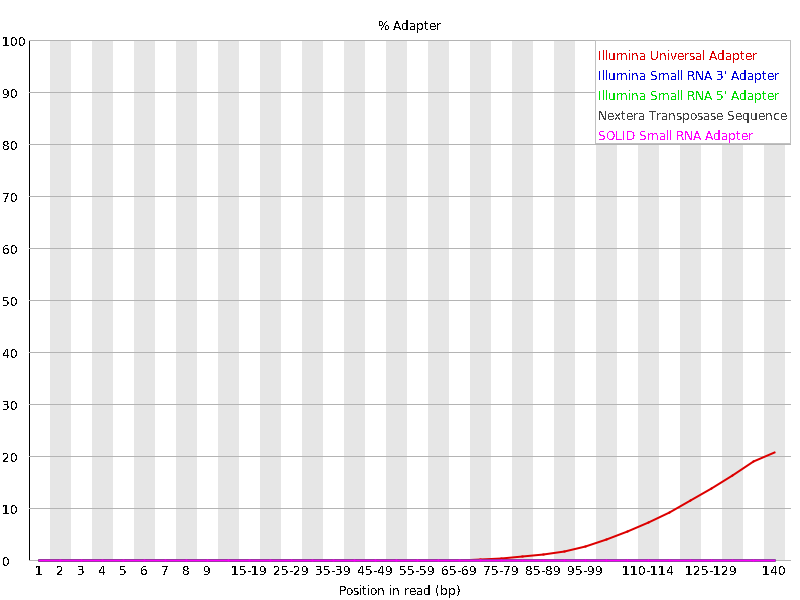
\includegraphics{./EarlyOnset_SRR21523117_pass_1_fastqc_adaptercontent.png}
2. Trim adapters using cutadapt

This study used the TruSeq Stranded mRNA LT Sample Prep Kit to prepare
samples.

According to the Illumina Adapter Sequences manual (Document \#
1000000002694 v17 pg. 48):
\url{https://support.illumina.com/downloads/illumina-adapter-sequences-document-1000000002694.html}

The sequence that can be used for TruSeq universal adapter trimming is:

AATGATACGGCGACCACCGAGATCTACACTCTTTCCCTACACGACGCTCTTCCGATCT

The authors were not clear about the adapter sequences they used, but
fastqc detected universal adapter sequences in this sample, so we will
assume they used this sequence and use cutadapt to trim it.

\begin{Shaded}
\begin{Highlighting}[]

\CommentTok{\# Trim adapters using cutadapt}

\VariableTok{sample}\OperatorTok{=}\NormalTok{EarlyOnset\_SRR21523117}

\ExtensionTok{cutadapt} \AttributeTok{{-}{-}cut}\NormalTok{ 10 }\AttributeTok{{-}a}\NormalTok{ AATGATACGGCGACCACCGAGATCTACACTCTTTCCCTACACGACGCTCTTCCGATCT }\AttributeTok{{-}o} \VariableTok{$sample}\NormalTok{.trimmed.\_pass\_1.fastq.gz }\VariableTok{$sample}\StringTok{"\_pass\_1.fastq.gz"}

\ExtensionTok{cutadapt} \AttributeTok{{-}{-}cut}\NormalTok{ 10 }\AttributeTok{{-}a}\NormalTok{ AATGATACGGCGACCACCGAGATCTACACTCTTTCCCTACACGACGCTCTTCCGATCT }\AttributeTok{{-}o} \VariableTok{$sample}\NormalTok{.trimmed.\_pass\_2.fastq.gz }\VariableTok{$sample}\StringTok{"\_pass\_2.fastq.gz"}

\CommentTok{\#Check the resulting fastq files for improvement in base quality}

\ExtensionTok{fastqc} \AttributeTok{{-}o}\NormalTok{ ./fastQC\_output }\VariableTok{$sample}\NormalTok{.trimmed.\_pass\_1.fastq.gz }\VariableTok{$sample}\NormalTok{.trimmed.\_pass\_2.fastq.gz}
\end{Highlighting}
\end{Shaded}

\begin{figure}
\centering
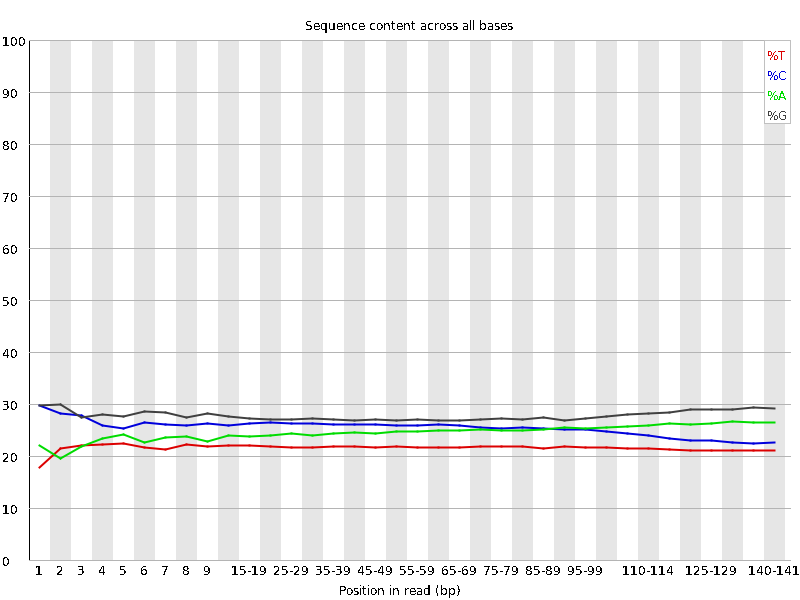
\includegraphics{./EarlyOnset_SRR21523117_pass_1_fastqc_basecontent_trimmed.png}
\caption{adapter content}
\end{figure}

Trimming improved the per base sequence content quality metric by
removing the first 10 bases from the reads in the fastqs (as shown
above), but the adapter content did not change, which means that a
different adapter sequence was used. Since we do not know what this
sequence was, we will move on and use the resulting trimmed fastqs for
subsequent steps.

\begin{enumerate}
\def\labelenumi{\arabic{enumi}.}
\setcounter{enumi}{2}
\tightlist
\item
  Align fastqs to hg38 reference genome using bowtie2 and convert to BAM
  file
\end{enumerate}

\begin{Shaded}
\begin{Highlighting}[]

\CommentTok{\# Paired{-}end alignment of trimmed fatsq files with the hg38 reference genome}

\VariableTok{sample}\OperatorTok{=}\NormalTok{EarlyOnset\_SRR21523117}

\ExtensionTok{bowtie2} \AttributeTok{{-}x}\NormalTok{ /projects/bmeg/indexes/hg38/hg38\_bowtie2\_index }\AttributeTok{{-}1} \VariableTok{$sample}\NormalTok{.trimmed.\_pass\_1.fastq.gz }\AttributeTok{{-}2} \VariableTok{$sample}\NormalTok{.trimmed.\_pass\_2.fastq.gz }\AttributeTok{{-}S} \VariableTok{$sample}\NormalTok{.aligned.sam}

\CommentTok{\# Sam to Bam conversion using samtools:}

\ExtensionTok{samtools}\NormalTok{ view }\AttributeTok{{-}h} \AttributeTok{{-}b} \AttributeTok{{-}o} \VariableTok{$sample}\NormalTok{.aligned.bam }\VariableTok{$sample}\NormalTok{.aligned.sam}
\end{Highlighting}
\end{Shaded}

\begin{enumerate}
\def\labelenumi{\arabic{enumi}.}
\setcounter{enumi}{3}
\tightlist
\item
  Produce a counts file using featureCounts
\end{enumerate}

After this step, we should have a text file that displays the number of
reads assigned to each given gene ID. This will tell us the expression
levels of each gene.

\begin{Shaded}
\begin{Highlighting}[]
\CommentTok{\#Download and unpack the subreads package}
\FunctionTok{wget} \AttributeTok{{-}{-}no{-}check{-}certificate}\NormalTok{ https://sourceforge.net/projects/subread/files/subread{-}2.0.4/subread{-}2.0.4{-}Linux{-}x86\_64.tar.gz}
\FunctionTok{tar}\NormalTok{ zxvf subread{-}2.0.4{-}Linux{-}x86\_64.tar.gz}

\CommentTok{\#Add the bin folder to the $PATH so we can use featureCounts}
\BuiltInTok{export} \VariableTok{PATH}\OperatorTok{=}\NormalTok{/home/lbrockley\_bmeg23/subread{-}2.0.4{-}Linux{-}x86\_64/bin:}\VariableTok{$PATH}

\CommentTok{\#Copy the hg38 annotation file in the subreads folder to the final project file to use for annotation with featurecounts}
\FunctionTok{cp}\NormalTok{ hg38\_RefSeq\_exon.txt /home/lbrockley\_bmeg23/final\_project/}
\CommentTok{\#Convert to the preferred file extension (saf)}
\FunctionTok{cp}\NormalTok{ hg38\_RefSeq\_exon.txt hg38\_RefSeq\_exon.saf}

\CommentTok{\#Summarize and count paired{-}end reads:}
\VariableTok{sample}\OperatorTok{=}\NormalTok{EarlyOnset\_SRR21523117}
\ExtensionTok{featureCounts} \AttributeTok{{-}p} \AttributeTok{{-}{-}countReadPairs} \AttributeTok{{-}t}\NormalTok{ exon }\AttributeTok{{-}g}\NormalTok{ gene\_id }\AttributeTok{{-}F} \StringTok{\textquotesingle{}SAF\textquotesingle{}} \AttributeTok{{-}a}\NormalTok{ hg38\_RefSeq\_exon.saf }\AttributeTok{{-}o} \VariableTok{$sample}\NormalTok{.counts.txt }\VariableTok{$sample}\NormalTok{.aligned.bam}
\end{Highlighting}
\end{Shaded}

The output of this script is a read counts file with 28397 rows:

\begin{Shaded}
\begin{Highlighting}[]
\NormalTok{EarlyOnset\_SRR21523117\_counts }\OtherTok{\textless{}{-}} \FunctionTok{read.csv}\NormalTok{(}\StringTok{\textquotesingle{}EarlyOnset\_SRR21523117.counts.csv\textquotesingle{}}\NormalTok{)}
\FunctionTok{head}\NormalTok{(EarlyOnset\_SRR21523117\_counts)}
\end{Highlighting}
\end{Shaded}

\begin{verbatim}
##      Geneid                                                    Chr
## 1 100287102                                         chr1;chr1;chr1
## 2    653635 chr1;chr1;chr1;chr1;chr1;chr1;chr1;chr1;chr1;chr1;chr1
## 3 102466751                                                   chr1
## 4 100302278                                                   chr1
## 5    645520                                         chr1;chr1;chr1
## 6     79501                                                   chr1
##                                                               Start
## 1                                                 11874;12613;13221
## 2 14362;14970;15796;16607;16858;17233;17606;17915;18268;24738;29321
## 3                                                             17369
## 4                                                             30366
## 5                                                 34611;35277;35721
## 6                                                             69091
##                                                                 End
## 1                                                 12227;12721;14409
## 2 14829;15038;15947;16765;17055;17368;17742;18061;18366;24891;29370
## 3                                                             17436
## 4                                                             30503
## 5                                                 35174;35481;36081
## 6                                                             70008
##                  Strand Length EarlyOnset_SRR21523117.aligned.bam
## 1                 +;+;+   1652                                  0
## 2 -;-;-;-;-;-;-;-;-;-;-   1769                                391
## 3                     -     68                                 13
## 4                     +    138                                  0
## 5                 -;-;-   1130                                  0
## 6                     +    918                                  0
\end{verbatim}

The featureCounts program states that a total of 56732052 alignments
occurred, and 21202936 (37.4\%) of alignments were successfully
assigned. It is likely that the performance of the alignment would have
been better if we had removed the correct adapter sequences using
cutadapt.

Once we had verified these steps for one sample, we incorporated them
into a pipeline.

We made a task file called sample\_names.txt, with the following
contents:

LateOnset\_SRR21523090 LateOnset\_SRR21523091 EarlyOnset\_SRR21523117
EarlyOnset\_SRR21523118

We used the script runTheseJobsSerially from assignment 2, made a
pipeline file called fastqToReadCounts.sh, and tested the pipeline as
follows:

\begin{Shaded}
\begin{Highlighting}[]
\CommentTok{\#\# Pipeline test}

\ExtensionTok{./runTheseJobsSerially.sh}\NormalTok{ ./fastqToBam.sh sample\_names.txt}
\end{Highlighting}
\end{Shaded}

\begin{Shaded}
\begin{Highlighting}[]
\CommentTok{\#\#fastqToBam pipeline}
\CommentTok{\#}
\BuiltInTok{set} \AttributeTok{{-}e} \CommentTok{\# this makes the whole script exit on any error.}
\VariableTok{sample}\OperatorTok{=}\VariableTok{$1}
\VariableTok{logDir}\OperatorTok{=}\NormalTok{MyLogDirectory }\CommentTok{\# this is where all the files to keep track of progress will go.}
\FunctionTok{mkdir} \AttributeTok{{-}p}\NormalTok{ MyLogDirectory }\CommentTok{\# make the directory where log files will go, if it doesn\textquotesingle{}t exist already}
\BuiltInTok{echo}\NormalTok{ running pipeline for }\VariableTok{$sample}
\CommentTok{\#}
\CommentTok{\# Trim adapters from the fastq files:}
\CommentTok{\#}
\CommentTok{\# QC: Check the quality of reads in the fastq files using fastQC}
\CommentTok{\#}
\ControlFlowTok{if} \BuiltInTok{[} \OtherTok{!} \OtherTok{{-}e} \VariableTok{$logDir}\NormalTok{/}\VariableTok{$sample}\NormalTok{.fastqc.done }\BuiltInTok{]} \CommentTok{\#run this code only if record of fastqc is missing}
\ControlFlowTok{then}
        \BuiltInTok{echo}\NormalTok{ Performing fastqc of sample }\VariableTok{$sample}\NormalTok{ with the following fastqs:}
        \FunctionTok{ls} \VariableTok{$sample}\StringTok{"\_pass\_1.fastq.gz"} \VariableTok{$sample}\StringTok{"\_pass\_2.fastq.gz"}
        \ExtensionTok{fastqc} \AttributeTok{{-}o}\NormalTok{ ./fastQC\_output }\VariableTok{$sample}\StringTok{"\_pass\_1.fastq.gz"} \VariableTok{$sample}\StringTok{"\_pass\_2.fastq.gz"}
        \FunctionTok{touch} \VariableTok{$logDir}\NormalTok{/}\VariableTok{$sample}\NormalTok{.fastqc.done }\CommentTok{\#create record to prevent repeating process on same file}
\ControlFlowTok{else} \CommentTok{\# $logDir/$sample.fastqc.done was not missing}
        \BuiltInTok{echo}\NormalTok{ Already performed fastqc of }\VariableTok{$sample}
\ControlFlowTok{fi}
\CommentTok{\#}
\CommentTok{\# Trim adapters using cutadapt:}
\CommentTok{\#}
\ControlFlowTok{if} \BuiltInTok{[} \OtherTok{!} \OtherTok{{-}e} \VariableTok{$logDir}\NormalTok{/}\VariableTok{$sample}\NormalTok{.trimming.done }\BuiltInTok{]} \CommentTok{\#run this code only if record is missing}
\ControlFlowTok{then}
        \BuiltInTok{echo}\NormalTok{ Performing cutadapt trim of sample }\VariableTok{$sample}\NormalTok{ with the following fastqs:}
        \FunctionTok{ls} \VariableTok{$sample}\StringTok{"\_pass\_1.fastq.gz"} \VariableTok{$sample}\StringTok{"\_pass\_2.fastq.gz"}
        \ExtensionTok{cutadapt} \AttributeTok{{-}{-}cut}\NormalTok{ 10 }\AttributeTok{{-}a}\NormalTok{ AATGATACGGCGACCACCGAGATCTACACTCTTTCCCTACACGACGCTCTTCCGATCT }\AttributeTok{{-}o} \VariableTok{$sample}\NormalTok{.trimmed.\_pass\_1.fastq.gz }\VariableTok{$sample}\StringTok{"\_pass\_1.fastq.gz"}
        \ExtensionTok{cutadapt} \AttributeTok{{-}{-}cut}\NormalTok{ 10 }\AttributeTok{{-}a}\NormalTok{ AATGATACGGCGACCACCGAGATCTACACTCTTTCCCTACACGACGCTCTTCCGATCT }\AttributeTok{{-}o} \VariableTok{$sample}\NormalTok{.trimmed.\_pass\_2.fastq.gz     }\VariableTok{$sample}\StringTok{"\_pass\_2.fastq.gz"}
        \FunctionTok{touch} \VariableTok{$logDir}\NormalTok{/}\VariableTok{$sample}\NormalTok{.trimming.done }\CommentTok{\#create record to prevent repeating process on same file}
\ControlFlowTok{else} \CommentTok{\# $logDir record was not missing}
        \BuiltInTok{echo}\NormalTok{ Already performed cutadapt trim of }\VariableTok{$sample}
\ControlFlowTok{fi}
\CommentTok{\#}
\CommentTok{\# Align reads to the hg38 reference genome using bowtie2 (the group used HISAT2 but these tools are comparable for RNASeq data):}
\CommentTok{\#}
\ControlFlowTok{if} \BuiltInTok{[} \OtherTok{!} \OtherTok{{-}e} \VariableTok{$logDir}\NormalTok{/}\VariableTok{$sample}\NormalTok{.alignment.done }\BuiltInTok{]} \CommentTok{\#run this code only if record of alignment is missing}
\ControlFlowTok{then}
        \BuiltInTok{echo}\NormalTok{ Performing bowtie2 alignment of sample }\VariableTok{$sample}\NormalTok{ with the following fastqs:}
        \FunctionTok{ls} \VariableTok{$sample}\StringTok{"\_pass\_1.fastq.gz"} \VariableTok{$sample}\StringTok{"\_pass\_2.fastq.gz"}
        \ExtensionTok{bowtie2} \AttributeTok{{-}x}\NormalTok{ /projects/bmeg/indexes/hg38/hg38\_bowtie2\_index }\AttributeTok{{-}1} \VariableTok{$sample}\NormalTok{.trimmed\_pass\_1.fastq.gz }\AttributeTok{{-}2} \VariableTok{$sample}\NormalTok{.trimmed.\_pass\_2.fastq.gz }\AttributeTok{{-}S} \VariableTok{$sample}\NormalTok{.alignment.sam}
        \FunctionTok{touch} \VariableTok{$logDir}\NormalTok{/}\VariableTok{$sample}\NormalTok{.alignment.done }\CommentTok{\#create record to prevent repeating process on same file}
\ControlFlowTok{else} \CommentTok{\# $logDir record was not missing}
        \BuiltInTok{echo}\NormalTok{ Already performed bowtie2 alignment of }\VariableTok{$sample}
\ControlFlowTok{fi}
\CommentTok{\#}
\CommentTok{\#Convert SAM files to BAM files using samtools view:}
\CommentTok{\#}
\ControlFlowTok{if} \BuiltInTok{[} \OtherTok{!} \OtherTok{{-}e} \VariableTok{$logDir}\NormalTok{/}\VariableTok{$sample}\NormalTok{.sam\_to\_bam.done }\BuiltInTok{]} \CommentTok{\#run this code only if record of conversion is missing}
\ControlFlowTok{then}
        \BuiltInTok{echo}\NormalTok{ Performing conversion of sample }\VariableTok{$sample}\NormalTok{ from .sam to .bam with the following .sam file:}
        \FunctionTok{ls} \VariableTok{$sample}\NormalTok{.alignment.sam}
        \ExtensionTok{samtools}\NormalTok{ view }\AttributeTok{{-}h} \AttributeTok{{-}b} \AttributeTok{{-}o} \VariableTok{$sample}\NormalTok{.alignment.bam }\VariableTok{$sample}\NormalTok{.alignment.sam}
        \FunctionTok{rm} \VariableTok{$sample}\NormalTok{.alignment.sam }\CommentTok{\#Remove the unnecessary sam file}
        \FunctionTok{touch} \VariableTok{$logDir}\NormalTok{/}\VariableTok{$sample}\NormalTok{.sam\_to\_bam.done }\CommentTok{\#create record to prevent repeating process on same file}
\ControlFlowTok{else} \CommentTok{\# $logDir record was not missing}
        \BuiltInTok{echo}\NormalTok{ Already performed conversion of .sam to .bam for }\VariableTok{$sample}
\ControlFlowTok{fi}
\CommentTok{\#}
\CommentTok{\# Count the aligned reads using featureCounts in the Subread 2.0.3 package:}
\CommentTok{\#}
\ControlFlowTok{if} \BuiltInTok{[} \OtherTok{!} \OtherTok{{-}e} \VariableTok{$logDir}\NormalTok{/}\VariableTok{$sample}\NormalTok{.featureCounts.done }\BuiltInTok{]} \CommentTok{\#run this code only if record is missing}
\ControlFlowTok{then}
        \BuiltInTok{echo}\NormalTok{ Counting features in }\VariableTok{$sample}\NormalTok{ in the following file:}
        \FunctionTok{ls} \VariableTok{$sample}\NormalTok{.alignment.sorted.filtered.bam }
        \ExtensionTok{featureCounts} \AttributeTok{{-}p} \AttributeTok{{-}{-}countReadPairs} \AttributeTok{{-}t}\NormalTok{ exon }\AttributeTok{{-}g}\NormalTok{ gene\_id }\AttributeTok{{-}o}\NormalTok{ counts.txt }\VariableTok{$sample}\NormalTok{.alignment.sorted.filtered.bam        }
        \FunctionTok{touch} \VariableTok{$logDir}\NormalTok{/}\VariableTok{$sample}\NormalTok{.featureCounts.done }\CommentTok{\#create record to prevent repeating process on same file}
\ControlFlowTok{else} \CommentTok{\# $logDir record was not missing}
        \BuiltInTok{echo}\NormalTok{ Already counted features for }\VariableTok{$sample}
\ControlFlowTok{fi}
\CommentTok{\#}
\BuiltInTok{echo}\NormalTok{ finished pipeline for }\VariableTok{$sample}
\end{Highlighting}
\end{Shaded}

We then ran featureCounts on all the BAM files generated.

\begin{Shaded}
\begin{Highlighting}[]
\ExtensionTok{featureCounts} \AttributeTok{{-}p} \AttributeTok{{-}{-}countReadPairs} \AttributeTok{{-}t}\NormalTok{ exon }\AttributeTok{{-}g}\NormalTok{ gene\_id }\AttributeTok{{-}F} \StringTok{\textquotesingle{}SAF\textquotesingle{}} \AttributeTok{{-}a}\NormalTok{ hg38\_RefSeq\_exon.saf }\AttributeTok{{-}o}\NormalTok{ counts.txt }\PreprocessorTok{*}\NormalTok{.bam}
\end{Highlighting}
\end{Shaded}

Part II: Analysis of read counts data to identify differentially
expressed genes (DEG) between early-onset and late-onset groups

To replicate the steps which produced the heatmap in Figure 1A and
volcano plot in Figure 2B, we use the read counts file available from
the GEO database that had been generated from all the fastq files. We
also compared plots produced using our filtered DEG list versus the
filtered DEG list provided in supplementary appendix 1 by the authors.

Part II A: Generating a normalized DEG list from the read counts file

\begin{Shaded}
\begin{Highlighting}[]
\FunctionTok{library}\NormalTok{(readr)}
\FunctionTok{library}\NormalTok{(dplyr)}
\end{Highlighting}
\end{Shaded}

\begin{verbatim}
## 
## Attaching package: 'dplyr'
\end{verbatim}

\begin{verbatim}
## The following objects are masked from 'package:stats':
## 
##     filter, lag
\end{verbatim}

\begin{verbatim}
## The following objects are masked from 'package:base':
## 
##     intersect, setdiff, setequal, union
\end{verbatim}

\begin{Shaded}
\begin{Highlighting}[]
\FunctionTok{library}\NormalTok{(tidyverse)}
\end{Highlighting}
\end{Shaded}

\begin{verbatim}
## -- Attaching core tidyverse packages ------------------------ tidyverse 2.0.0 --
## v forcats   1.0.0     v stringr   1.5.0
## v ggplot2   3.4.1     v tibble    3.2.1
## v lubridate 1.9.2     v tidyr     1.3.0
## v purrr     1.0.1
\end{verbatim}

\begin{verbatim}
## -- Conflicts ------------------------------------------ tidyverse_conflicts() --
## x dplyr::filter() masks stats::filter()
## x dplyr::lag()    masks stats::lag()
## i Use the ]8;;http://conflicted.r-lib.org/conflicted package]8;; to force all conflicts to become errors
\end{verbatim}

\begin{Shaded}
\begin{Highlighting}[]
\CommentTok{\# Store the RNAseq read counts file as a dataframe}
\NormalTok{counts\_data }\OtherTok{\textless{}{-}} \FunctionTok{read\_tsv}\NormalTok{(}\StringTok{\textquotesingle{}GSE213092\_HRCRC\_rowsort.txt\textquotesingle{}}\NormalTok{)}
\end{Highlighting}
\end{Shaded}

\begin{verbatim}
## Rows: 33125 Columns: 100
## -- Column specification --------------------------------------------------------
## Delimiter: "\t"
## chr  (1): Gene
## dbl (99): HRCRC2004, HRCRC2021, HRCRC2039, HRCRC2045, HRCRC2047, HRCRC2049, ...
## 
## i Use `spec()` to retrieve the full column specification for this data.
## i Specify the column types or set `show_col_types = FALSE` to quiet this message.
\end{verbatim}

\begin{Shaded}
\begin{Highlighting}[]
\NormalTok{counts\_data }\OtherTok{\textless{}{-}} \FunctionTok{as.data.frame}\NormalTok{(counts\_data)}
\NormalTok{counts\_data }\OtherTok{\textless{}{-}}\NormalTok{ counts\_data[}\SpecialCharTok{!}\FunctionTok{rowSums}\NormalTok{(}\FunctionTok{is.na}\NormalTok{(counts\_data)),] }\CommentTok{\#Remove NA values from counts data}

\CommentTok{\#NOTE: There were duplicate rows for genes labelled "01{-}Mar" and "02{-}Mar" in the original data.}
\CommentTok{\#These seemed to be mislabeled, and were causing issues with downstream steps, so we decided to remove these rows.}
\CommentTok{\#Ideally, we would find out why these genes were mislabeled and correctly identify them, but we do not have enough information to do that.}
\NormalTok{counts\_data }\OtherTok{\textless{}{-}}\NormalTok{ counts\_data[counts\_data}\SpecialCharTok{$}\NormalTok{Gene }\SpecialCharTok{!=} \StringTok{"01{-}Mar"}\NormalTok{, ]}
\NormalTok{counts\_data }\OtherTok{\textless{}{-}}\NormalTok{ counts\_data[counts\_data}\SpecialCharTok{$}\NormalTok{Gene }\SpecialCharTok{!=} \StringTok{"02{-}Mar"}\NormalTok{, ]}

\CommentTok{\#Set the row names to be the gene names}
\FunctionTok{row.names}\NormalTok{(counts\_data) }\OtherTok{\textless{}{-}}\NormalTok{ counts\_data[,}\DecValTok{1}\NormalTok{]}
\NormalTok{counts\_data }\OtherTok{\textless{}{-}}\NormalTok{ counts\_data[, }\SpecialCharTok{{-}}\DecValTok{1}\NormalTok{]}

\CommentTok{\# Convert the counts data into a format that DGEList will accept: integer matrix}
\NormalTok{dge\_counts }\OtherTok{\textless{}{-}} \FunctionTok{as.matrix}\NormalTok{(counts\_data)}
\FunctionTok{mode}\NormalTok{(dge\_counts) }\OtherTok{\textless{}{-}}\StringTok{"integer"}

\CommentTok{\#Read in a table of sample labels, so each sample can be matched to disease state (early or late onset colon cancer)}
\NormalTok{sample\_labels }\OtherTok{\textless{}{-}} \FunctionTok{read.csv}\NormalTok{(}\StringTok{\textquotesingle{}sample\_labels.csv\textquotesingle{}}\NormalTok{)}
\NormalTok{sample\_labels }\OtherTok{\textless{}{-}}\NormalTok{ sample\_labels[}\SpecialCharTok{!}\FunctionTok{rowSums}\NormalTok{(}\FunctionTok{is.na}\NormalTok{(sample\_labels)),] }\CommentTok{\#Remove NA values}
\NormalTok{sample\_labels\_subset }\OtherTok{\textless{}{-}}\NormalTok{ sample\_labels[, }\FunctionTok{c}\NormalTok{(}\DecValTok{8}\NormalTok{,}\DecValTok{16}\NormalTok{)] }\CommentTok{\# Create list of sample names with early vs late onset, to be used later for the heatmap}
\NormalTok{sample\_labels\_subset }\OtherTok{\textless{}{-}}\NormalTok{ sample\_labels\_subset[}\FunctionTok{order}\NormalTok{(sample\_labels\_subset}\SpecialCharTok{$}\NormalTok{disease\_state),] }\CommentTok{\# Sort the list}
\NormalTok{sample\_labels\_subset}\SpecialCharTok{$}\NormalTok{EorL }\OtherTok{\textless{}{-}} \FunctionTok{c}\NormalTok{(}\FunctionTok{as.numeric}\NormalTok{(sample\_labels\_subset}\SpecialCharTok{$}\NormalTok{disease\_state }\SpecialCharTok{==} \StringTok{"Early{-}onset colorectal cancer"}\NormalTok{)) }\CommentTok{\#Used for sample labelling in the later heatmap}

\CommentTok{\# Normalize read counts for every gene with the trimmed mean of M{-}values (TMM) method, using the edgeR package to create a DGEList object.}
\CommentTok{\# 2 disease state groups: early{-}onset and late{-}onset colon cancer}
\FunctionTok{library}\NormalTok{(edgeR)}
\end{Highlighting}
\end{Shaded}

\begin{verbatim}
## Loading required package: limma
\end{verbatim}

\begin{Shaded}
\begin{Highlighting}[]
\NormalTok{dge }\OtherTok{\textless{}{-}} \FunctionTok{DGEList}\NormalTok{(}\AttributeTok{counts=}\NormalTok{dge\_counts, }\AttributeTok{samples =} \FunctionTok{as.data.frame}\NormalTok{(}\FunctionTok{colnames}\NormalTok{(dge\_counts)), }\AttributeTok{genes =} \FunctionTok{rownames}\NormalTok{(counts\_data), }\AttributeTok{group =}\NormalTok{ sample\_labels}\SpecialCharTok{$}\NormalTok{disease\_state)}
\NormalTok{dge }\OtherTok{\textless{}{-}} \FunctionTok{calcNormFactors}\NormalTok{(dge, }\AttributeTok{method =} \StringTok{"TMM"}\NormalTok{)}
\NormalTok{dge\_counts\_normalized }\OtherTok{\textless{}{-}} \FunctionTok{cpm}\NormalTok{(dge, }\AttributeTok{log=}\ConstantTok{TRUE}\NormalTok{) }\CommentTok{\# Data frame of read counts normalized based on CPM and the TMM normalization factors, converted to log2}
\NormalTok{dge\_counts\_normalized\_z\_scores }\OtherTok{\textless{}{-}} \FunctionTok{apply}\NormalTok{(dge\_counts\_normalized, }\DecValTok{2}\NormalTok{, }\ControlFlowTok{function}\NormalTok{(x) (x }\SpecialCharTok{{-}} \FunctionTok{mean}\NormalTok{(x)) }\SpecialCharTok{/} \FunctionTok{sd}\NormalTok{(x)) }\CommentTok{\# Calculating Z{-}score for the counts}

\CommentTok{\#Create GLM model for differential gene expression comparison}
\NormalTok{design }\OtherTok{\textless{}{-}} \FunctionTok{model.matrix}\NormalTok{(}\SpecialCharTok{\textasciitilde{}}\NormalTok{sample\_labels}\SpecialCharTok{$}\NormalTok{disease\_state)}
\NormalTok{dge }\OtherTok{=} \FunctionTok{estimateDisp}\NormalTok{(dge, design)}
\NormalTok{fit }\OtherTok{=} \FunctionTok{glmQLFit}\NormalTok{(dge, design)}
\NormalTok{qlf }\OtherTok{=} \FunctionTok{glmQLFTest}\NormalTok{(fit, }\AttributeTok{coef=}\DecValTok{2}\NormalTok{) }
\FunctionTok{topTags}\NormalTok{(qlf, }\AttributeTok{n=}\DecValTok{10}\NormalTok{, }\AttributeTok{adjust.method=}\StringTok{"BH"}\NormalTok{, }\AttributeTok{sort.by=}\StringTok{"logFC"}\NormalTok{, }\AttributeTok{p.value=}\FloatTok{0.01}\NormalTok{) }\CommentTok{\#Checking output}
\end{Highlighting}
\end{Shaded}

\begin{verbatim}
## Coefficient:  sample_labels$disease_stateLate-onset colorectal cancer 
##                     genes     logFC       logCPM        F       PValue
## LYPD2               LYPD2  8.039594  1.864510647 63.78128 2.207443e-12
## CT45A1             CT45A1 -7.672155 -0.784735525 37.81708 1.057839e-07
## TRIML2             TRIML2 -7.427931  0.448210181 62.25712 3.559765e-12
## TTC29               TTC29 -7.167569  0.794038748 65.69094 1.220804e-12
## FAM41C             FAM41C -6.979214 -0.496674013 66.62922 9.148810e-13
## SFTA3               SFTA3 -6.796528  1.324604075 51.47171 1.202254e-10
## TSIX                 TSIX  6.693675  2.160305276 50.08662 1.924976e-10
## MROH2B             MROH2B -6.614226  0.182458904 52.73837 7.847643e-11
## LIPF                 LIPF -6.486915  0.003640786 51.73683 1.099228e-10
## LOC102546175 LOC102546175 -5.975548 -1.740517102 63.29465 2.570003e-12
##                       FDR
## LYPD2        2.127641e-08
## CT45A1       6.255418e-05
## TRIML2       2.357632e-08
## TTC29        2.021346e-08
## FAM41C       2.021346e-08
## SFTA3        2.654175e-07
## TSIX         3.984098e-07
## MROH2B       2.362497e-07
## LIPF         2.600066e-07
## LOC102546175 2.127641e-08
\end{verbatim}

\begin{Shaded}
\begin{Highlighting}[]
\CommentTok{\# Calculating FDR values for all the P{-}values using the same method as topTags}
\NormalTok{dge\_fdr }\OtherTok{\textless{}{-}} \FunctionTok{as.data.frame}\NormalTok{(}\FunctionTok{p.adjust}\NormalTok{(qlf}\SpecialCharTok{$}\NormalTok{table}\SpecialCharTok{$}\NormalTok{PValue, }\AttributeTok{method =} \StringTok{"BH"}\NormalTok{))}
\FunctionTok{colnames}\NormalTok{(dge\_fdr) }\OtherTok{\textless{}{-}} \FunctionTok{c}\NormalTok{(}\StringTok{"FDR"}\NormalTok{)}

\CommentTok{\# Creating a data frame of the DGE data that can be filtered as specified in the paper}
\NormalTok{dge\_fc }\OtherTok{\textless{}{-}} \FunctionTok{c}\NormalTok{(qlf}\SpecialCharTok{$}\NormalTok{genes, qlf}\SpecialCharTok{$}\NormalTok{table, dge\_fdr)}
\NormalTok{dge\_fc }\OtherTok{\textless{}{-}} \FunctionTok{data.frame}\NormalTok{(dge\_fc)}
\NormalTok{dge\_fc[,}\DecValTok{2}\NormalTok{] }\OtherTok{\textless{}{-}}\NormalTok{ dge\_fc[,}\DecValTok{2}\NormalTok{] }\SpecialCharTok{*} \SpecialCharTok{{-}}\DecValTok{1} \CommentTok{\# The paper\textquotesingle{}s supplementary table had fold{-}change values with opposite sign because FC comparison had been made in the opposite direction.}

\CommentTok{\# Filter DGE data based on following criteria: }
\CommentTok{\# p \textless{} 0.01, |log2FC| \textgreater{}1, logCPM \textgreater{} 1}
\NormalTok{dge\_fc\_filtered }\OtherTok{\textless{}{-}}\NormalTok{ dge\_fc[}\FunctionTok{which}\NormalTok{(dge\_fc}\SpecialCharTok{$}\NormalTok{PValue }\SpecialCharTok{\textless{}} \FloatTok{0.01}\NormalTok{),]}
\NormalTok{dge\_fc\_filtered }\OtherTok{\textless{}{-}}\NormalTok{ dge\_fc\_filtered[}\FunctionTok{which}\NormalTok{(dge\_fc\_filtered}\SpecialCharTok{$}\NormalTok{logCPM }\SpecialCharTok{\textgreater{}} \DecValTok{1}\NormalTok{),]}
\NormalTok{dge\_fc\_filtered }\OtherTok{\textless{}{-}}\NormalTok{ dge\_fc\_filtered[}\FunctionTok{which}\NormalTok{(}\FunctionTok{abs}\NormalTok{(dge\_fc\_filtered}\SpecialCharTok{$}\NormalTok{logFC) }\SpecialCharTok{\textgreater{}} \DecValTok{1}\NormalTok{),]}
\CommentTok{\#This narrowed the list of candidate genes from 33119 to 142}

\CommentTok{\# Sort based on fold change values}
\NormalTok{dge\_fc\_filtered }\OtherTok{\textless{}{-}}\NormalTok{ dge\_fc\_filtered[}\FunctionTok{order}\NormalTok{(}\SpecialCharTok{{-}}\NormalTok{dge\_fc\_filtered}\SpecialCharTok{$}\NormalTok{logFC),]}

\CommentTok{\# The authors have made their filtered DGE gene list available in supplementary appendix 1.}
\NormalTok{paper\_dge\_fc }\OtherTok{\textless{}{-}} \FunctionTok{read.csv}\NormalTok{(}\StringTok{\textquotesingle{}cam45675{-}sup{-}0001{-}appendixs1.csv\textquotesingle{}}\NormalTok{)}
\end{Highlighting}
\end{Shaded}

\begin{Shaded}
\begin{Highlighting}[]
\NormalTok{paper\_dge\_fc }\CommentTok{\# Authors\textquotesingle{} filtered DEG list}
\end{Highlighting}
\end{Shaded}

\begin{verbatim}
##               Gene     logFC   logCPM      Pvalue         FDR
## 1             DKK1  3.058917 2.651100 0.000011900 0.009293639
## 2             CPS1  3.056194 4.160139 0.000003510 0.005028720
## 3              FST  2.818496 3.046420 0.000010800 0.008999947
## 4            DHRS2  2.750514 3.875092 0.000000282 0.003285368
## 5            VSIG1  2.747192 1.414434 0.000005830 0.006133218
## 6            VENTX  2.538862 1.956859 0.000001250 0.003285368
## 7            IGFL2  2.277510 2.383304 0.000570426 0.051183613
## 8        LINC00176  2.194743 3.640655 0.000588977 0.051508496
## 9            CCL19  2.033946 2.608557 0.000237184 0.038572909
## 10           CXCL5  2.027958 6.743508 0.008052132 0.136583201
## 11            ODAM  1.939313 3.337928 0.000648343 0.053256806
## 12            CHGB  1.922057 1.135994 0.000760739 0.056875189
## 13            IL1A  1.885146 2.145483 0.000067800 0.021872377
## 14            GLDC  1.883084 2.216823 0.000539823 0.050388840
## 15          PRKAA2  1.851913 1.752601 0.000459885 0.047343824
## 16              C7  1.819364 3.073255 0.001590329 0.076899715
## 17           LYVE1  1.784610 2.039841 0.000765582 0.056883094
## 18           ADH1B  1.720362 2.510201 0.004600816 0.109634255
## 19            IGF1  1.648715 2.737529 0.004104493 0.105442637
## 20    RP11-279F6.1  1.602008 1.896859 0.002542859 0.089379764
## 21           WASF3  1.540132 2.490754 0.000438823 0.047343824
## 22            AOX1  1.498411 1.796540 0.000425745 0.047343824
## 23             MME  1.461033 4.625275 0.000804315 0.058202168
## 24          CXCL13  1.404778 3.311023 0.004719423 0.110458312
## 25            MED1  1.382170 6.211808 0.000002570 0.004996644
## 26          ADAM23  1.370648 1.356662 0.000851477 0.060205934
## 27           BNIP3  1.358201 4.982358 0.000647903 0.053256806
## 28           FSIP1  1.354895 1.485771 0.001606365 0.076899715
## 29            OXTR  1.324941 2.163130 0.000138120 0.031508021
## 30          FGFBP1  1.289092 3.962569 0.000451723 0.047343824
## 31         C3orf14  1.263725 1.942435 0.001127290 0.065423279
## 32          RPL39L  1.259531 2.681598 0.001272462 0.069698231
## 33            CST7  1.247194 2.714671 0.001528776 0.076317845
## 34           OLFM1  1.235849 2.766260 0.002925770 0.093892125
## 35            SRPX  1.167997 2.109892 0.000900585 0.061196027
## 36           LETM2  1.155515 1.695894 0.000571050 0.051183613
## 37            GRB7  1.149826 6.017528 0.000141811 0.031508021
## 38             CPM  1.146831 3.860273 0.000660478 0.053256806
## 39           CERS4  1.112631 2.522220 0.001744694 0.078862412
## 40           PGAP3  1.105070 6.226750 0.000319001 0.044142502
## 41            SIT1  1.100930 2.111198 0.002879952 0.093772939
## 42            MAP9  1.083404 2.387816 0.006923135 0.128176523
## 43           PTPRU  1.066390 3.828514 0.005125722 0.114847357
## 44           CDK12  1.058102 6.602587 0.000018100 0.012993341
## 45            SELL  1.000293 2.845628 0.009688284 0.145351891
## 46           PLIN5 -1.002079 1.100494 0.009429417 0.144518238
## 47           PRR22 -1.026002 2.814064 0.000250424 0.039204770
## 48            TFF3 -1.037110 9.699850 0.002960314 0.093892125
## 49           HSPA2 -1.038062 4.339319 0.000483016 0.048225211
## 50           RAB26 -1.040716 2.768909 0.005728646 0.121060794
## 51        PPP1R14A -1.045339 3.714023 0.008741997 0.140565516
## 52         CACNA1H -1.051080 4.172806 0.001391579 0.072930785
## 53            SHC3 -1.053232 2.160678 0.001613553 0.076899715
## 54    LOC101928262 -1.059580 1.549218 0.002659010 0.091385370
## 55        C10orf11 -1.059637 2.144226 0.000908389 0.061236797
## 56           CPNE7 -1.070068 6.475228 0.004384399 0.108511351
## 57  RP11-277P12.20 -1.084417 2.429604 0.005639334 0.120231923
## 58           P2RX1 -1.087330 1.460731 0.006653360 0.127242401
## 59            MYL9 -1.093166 7.734980 0.006677936 0.127242401
## 60           AIFM3 -1.094979 6.161154 0.001026810 0.064023443
## 61          CCDC78 -1.097769 3.095817 0.001249099 0.068897001
## 62           INHBB -1.104988 2.573333 0.001168013 0.066993279
## 63          CAPN12 -1.109484 4.951363 0.000112369 0.028590659
## 64           DUOX1 -1.121146 1.925714 0.004321330 0.108455746
## 65          CYP2D6 -1.127596 2.314671 0.000526875 0.049769141
## 66    LOC102724312 -1.143981 1.351404 0.001008257 0.063367533
## 67           RASD2 -1.156550 2.171868 0.000132237 0.031256117
## 68            GATM -1.158357 3.593447 0.000735078 0.055913712
## 69            TPM2 -1.174622 7.940233 0.000903878 0.061196027
## 70         LRRC16B -1.181146 2.371706 0.000037100 0.015394289
## 71           PDE4C -1.195361 2.257044 0.002835773 0.093772939
## 72    LOC100288152 -1.216635 4.761460 0.000384978 0.046209513
## 73        MIR143HG -1.230220 1.222365 0.004810783 0.111112897
## 74        C16orf54 -1.262153 1.465266 0.007970711 0.135639669
## 75         LGALS9B -1.274949 2.819566 0.001225576 0.068292157
## 76         TMPRSS5 -1.279830 1.602911 0.003617228 0.101533412
## 77         TMEM158 -1.332893 4.026107 0.000005070 0.005710247
## 78         TMEM249 -1.368068 2.217303 0.004192203 0.107009706
## 79            TMC8 -1.370581 4.941911 0.000033500 0.015223838
## 80           CPLX2 -1.384677 1.251766 0.005732641 0.121060794
## 81           MARCO -1.387430 1.271942 0.009512092 0.144638801
## 82          ADAM33 -1.400388 2.742547 0.007832739 0.134745327
## 83          AXDND1 -1.423863 1.372933 0.000950127 0.061427245
## 84         C2orf82 -1.431264 4.638041 0.000030500 0.014949766
## 85           WFDC2 -1.484012 5.442301 0.001065977 0.064231434
## 86            TCN1 -1.513772 3.822259 0.007050590 0.128581561
## 87       FEZF1-AS1 -1.519951 3.004160 0.006284631 0.125680901
## 88           RASD1 -1.525540 3.932389 0.000538584 0.050388840
## 89       LINC00261 -1.532248 5.172525 0.000769766 0.056883094
## 90           FOXH1 -1.535327 1.852069 0.000797398 0.058202168
## 91        MTRNR2L8 -1.541452 1.743184 0.002170648 0.083926398
## 92             NPW -1.574873 2.214730 0.004383252 0.108511351
## 93   RP11-234B24.2 -1.589082 4.246457 0.000067900 0.021872377
## 94             HBB -1.606411 3.589303 0.002376881 0.087605844
## 95          DUOXA1 -1.679470 1.275457 0.000334079 0.044410883
## 96           BMPER -1.684303 1.297608 0.000336547 0.044410883
## 97          PRSS33 -1.778008 2.721264 0.000248133 0.039204770
## 98            ALPL -1.786826 2.451849 0.000012400 0.009293639
## 99           ANPEP -1.788250 6.840263 0.000437347 0.047343824
## 100           RBP4 -1.820431 3.885243 0.000135622 0.031462256
## 101          KLK12 -1.850545 2.636538 0.000354367 0.045080559
## 102        COL11A2 -1.924202 1.752820 0.000006710 0.006613639
## 103      TNFRSF11B -1.950348 4.005959 0.000002420 0.004996644
## 104         PCDH19 -1.978111 1.702850 0.000091400 0.026696923
## 105        CCDC88B -1.981791 7.381796 0.000001150 0.003285368
## 106         GALNT8 -1.988366 4.276753 0.000462931 0.047343824
## 107          JSRP1 -2.011486 2.149304 0.000001030 0.003285368
## 108            GIF -2.047887 1.446718 0.000509590 0.049626070
## 109         SPINK4 -2.087743 7.110221 0.000961448 0.061653819
## 110           PSCA -2.128209 2.008705 0.000438605 0.047343824
## 111           DKK4 -2.153866 2.197259 0.000688984 0.053805520
## 112           SOX1 -2.227941 1.531231 0.000588491 0.051508496
## 113         S100A3 -2.250243 2.245634 0.000000837 0.003285368
## 114          EPHA7 -2.272059 1.953914 0.000109945 0.028590659
## 115         S100A1 -2.326194 1.684741 0.000023100 0.013831994
## 116         ELK2AP -2.453198 4.960802 0.000274972 0.041376562
## 117          TRNS1 -2.663558 3.728968 0.000194279 0.035319564
## 118          KCNA6 -2.673340 2.521951 0.000001100 0.003285368
## 119          PCSK1 -2.708236 4.966611 0.000312913 0.043683231
## 120          PRSS2 -2.736963 2.453020 0.000129227 0.031256117
## 121           TFF2 -3.147768 4.198669 0.000003170 0.004996644
## 122            NTS -3.405769 6.367031 0.000669606 0.053256806
\end{verbatim}

\begin{Shaded}
\begin{Highlighting}[]
\NormalTok{dge\_fc\_filtered }\CommentTok{\#Our filtered DEG list.}
\end{Highlighting}
\end{Shaded}

\begin{verbatim}
##                genes     logFC   logCPM         F       PValue          FDR
## 8407           SFTA3  6.796528 1.324604 51.471705 1.202254e-10 2.654175e-07
## 17185          SFTPB  5.954527 1.717038 51.884740 1.045710e-10 2.600066e-07
## 29732          SFRP1  3.587512 2.276326 25.184993 2.218240e-06 6.278378e-04
## 7049          SLC5A8  3.510088 1.207565 20.082961 1.946316e-05 3.025927e-03
## 18076           CPS1  3.106382 4.163989 25.038783 2.357256e-06 6.505046e-04
## 3439            DKK1  3.093399 2.689423 21.494318 1.055845e-05 2.044696e-03
## 23094         ANXA10  2.964493 2.357703 13.292112 4.218674e-04 2.925329e-02
## 23534            FST  2.851120 3.077687 21.839173 9.104672e-06 1.805397e-03
## 8408          NKX2-1  2.845533 3.479121 10.286331 1.791587e-03 7.071325e-02
## 8296           DHRS2  2.815555 3.869155 32.263730 1.282314e-07 7.121293e-05
## 11556       SLC22A31  2.799027 3.088809 15.696353 1.381354e-04 1.317233e-02
## 32528          VSIG1  2.794325 1.467187 22.967947 5.625836e-06 1.293747e-03
## 22617      LINC01088  2.764546 1.109157 23.923492 3.757987e-06 9.572749e-04
## 14771   LOC102724908  2.729870 2.069564 10.711454 1.454636e-03 6.329865e-02
## 4158           VENTX  2.522386 1.942274 26.351850 1.369586e-06 4.403285e-04
## 31067            OGN  2.458349 1.754858 11.226747 1.132007e-03 5.432814e-02
## 4249            MUC6  2.392432 2.505474  8.907928 3.555236e-03 1.044646e-01
## 15236          IGFL2  2.327226 2.376316 13.285716 4.231414e-04 2.925329e-02
## 32474           NXF3  2.243322 1.451453 10.791543 1.398857e-03 6.200204e-02
## 19215      LINC00176  2.155823 3.576379 12.450376 6.286824e-04 3.799054e-02
## 30724          CCL19  2.055129 2.644090 14.638523 2.248498e-04 1.949189e-02
## 5554          WTAPP1  2.045367 1.179295  8.011183 5.601876e-03 1.313783e-01
## 22564          CXCL5  2.016141 6.754042  7.246799 8.305250e-03 1.611961e-01
## 15109         CXCL17  2.013007 1.877251  8.903649 3.562896e-03 1.045969e-01
## 22527           ODAM  1.967313 3.356242 12.723804 5.520014e-04 3.481815e-02
## 17456           IL1A  1.900332 2.150864 17.480965 6.153850e-05 7.410354e-03
## 18545           CHGB  1.894356 1.125182 11.473005 1.004828e-03 5.049301e-02
## 30567           GLDC  1.879186 2.220815 12.665278 5.675636e-04 3.546202e-02
## 23485             C7  1.831098 3.078627 10.695644 1.465915e-03 6.363703e-02
## 989           PRKAA2  1.825559 1.744923 12.613150 5.818042e-04 3.614718e-02
## 18633          INSM1  1.798939 1.032704  9.568873 2.554543e-03 8.694111e-02
## 4495           LYVE1  1.778461 2.050905 11.887238 8.230731e-04 4.453606e-02
## 22731          ADH1B  1.705516 2.522685  8.209587 5.062469e-03 1.249609e-01
## 7064            IGF1  1.660342 2.744002  8.755489 3.838929e-03 1.089341e-01
## 9842    RP11-279F6.1  1.571786 1.853556  9.357474 2.838275e-03 9.107506e-02
## 7588           WASF3  1.554230 2.487588 13.490147 3.843171e-04 2.766665e-02
## 17974           AOX1  1.502487 1.809446 13.151979 4.506998e-04 3.020982e-02
## 21659            MME  1.443198 4.628114 11.645675 9.245058e-04 4.806124e-02
## 22606         CXCL13  1.433300 3.346441  8.586703 4.180539e-03 1.135298e-01
## 12437           MED1  1.400340 6.227877 25.046688 2.349518e-06 6.505046e-04
## 9464           FSIP1  1.394861 1.472526 11.217709 1.136978e-03 5.433442e-02
## 4139           BNIP3  1.392211 4.974904 13.200004 4.405974e-04 2.977629e-02
## 20469           OXTR  1.367552 2.168658 16.684247 8.811413e-05 9.535619e-03
## 18033         ADAM23  1.357468 1.355360 11.511826 9.861647e-04 5.003485e-02
## 22270         FGFBP1  1.353682 3.975770 14.494763 2.403560e-04 2.003779e-02
## 21051        C3orf14  1.281350 1.945473 11.491581 9.958530e-04 5.038669e-02
## 21890         RPL39L  1.276979 2.685472 11.272945 1.106944e-03 5.359128e-02
## 18673           CST7  1.275597 2.735093 10.963022 1.286716e-03 5.877189e-02
## 31609          OLFM1  1.258598 2.788802  9.517843 2.620235e-03 8.770832e-02
## 12448           GRB7  1.201405 6.016581 17.329488 6.586910e-05 7.818120e-03
## 29712          LETM2  1.194781 1.707662 13.328383 4.147182e-04 2.903466e-02
## 32037           SRPX  1.167615 2.123879 11.482189 1.000381e-03 5.038669e-02
## 12444          PGAP3  1.148656 6.230081 15.105746 1.811801e-04 1.648291e-02
## 6863             CPM  1.123813 3.846572 12.020668 7.720277e-04 4.331524e-02
## 14317          CERS4  1.105369 2.503410 10.380549 1.710542e-03 6.899464e-02
## 30746           SIT1  1.095820 2.099205  9.307144 2.910504e-03 9.231930e-02
## 590            PTPRU  1.083183 3.842465  8.389671 4.619481e-03 1.197094e-01
## 12438          CDK12  1.082095 6.611239 20.956055 1.331855e-05 2.384021e-03
## 23039           MAP9  1.069445 2.383834  7.399371 7.673692e-03 1.538222e-01
## 5272    LOC101928262 -1.005617 1.518965  8.611856 4.127699e-03 1.126865e-01
## 10433        CACNA1H -1.006551 4.164819  9.956421 2.107987e-03 7.764848e-02
## 14957       PPP1R14A -1.011740 3.676074  6.916616 9.864384e-03 1.713846e-01
## 10417         CCDC78 -1.013125 3.034094  9.956835 2.107556e-03 7.764848e-02
## 8599           HSPA2 -1.021445 4.340159 12.554256 5.983358e-04 3.689738e-02
## 11764          P2RX1 -1.025081 1.443342  6.892567 9.989254e-03 1.721093e-01
## 9587           DUOX1 -1.041773 1.899666  7.424197 7.575749e-03 1.527838e-01
## 18826           MYL9 -1.044394 7.709637  7.130137 8.824524e-03 1.666083e-01
## 6196  RP11-277P12.20 -1.056385 2.431010  7.552796 7.088811e-03 1.478432e-01
## 17513          INHBB -1.059327 2.563249 10.290784 1.787669e-03 7.064279e-02
## 20182         CYP2D6 -1.062305 2.264972 11.926781 8.075933e-04 4.430485e-02
## 14972         CAPN12 -1.070239 4.925164 15.532853 1.488798e-04 1.396644e-02
## 8303         LRRC16B -1.085919 2.312893 16.876607 8.077533e-05 9.067373e-03
## 72      LOC102724312 -1.089961 1.309923 10.754599 1.424307e-03 6.222419e-02
## 20017          RASD2 -1.109351 2.162124 14.535857 2.358147e-04 2.001609e-02
## 30751           TPM2 -1.132969 7.911359 11.162546 1.167812e-03 5.493195e-02
## 9594            GATM -1.140559 3.594916 11.731117 8.872339e-04 4.656251e-02
## 14651          PDE4C -1.164390 2.246212  8.926771 3.521708e-03 1.040333e-01
## 23269   LOC100288152 -1.165414 4.711353 13.006513 4.827771e-04 3.166075e-02
## 24276       MIR143HG -1.188486 1.207084  7.854861 6.068710e-03 1.375701e-01
## 12141        LGALS9B -1.211401 2.796500 10.119850 1.944616e-03 7.396418e-02
## 5652         TMPRSS5 -1.217451 1.567788  8.160967 5.189463e-03 1.262668e-01
## 10903       C16orf54 -1.235654 1.476480  6.909048 9.903504e-03 1.716362e-01
## 13198           TMC8 -1.239202 4.865442 16.520189 9.491177e-05 1.006374e-02
## 30389        TMEM249 -1.239408 2.092588  7.526237 7.186638e-03 1.486481e-01
## 20771        TMEM158 -1.256718 3.990512 21.436065 1.082653e-05 2.060462e-03
## 18288        C2orf82 -1.341181 4.580980 17.590963 5.857745e-05 7.079534e-03
## 2306          AXDND1 -1.362348 1.360946 10.508402 1.606567e-03 6.650185e-02
## 24471          CPLX2 -1.389059 1.257524  7.808558 6.214605e-03 1.393342e-01
## 17497          MARCO -1.401910 1.304170  6.895014 9.976472e-03 1.720001e-01
## 18943          WFDC2 -1.426517 5.412546 10.662119 1.490132e-03 6.381674e-02
## 30404          FOXH1 -1.453615 1.786784 11.085057 1.212586e-03 5.647647e-02
## 18646      LINC00261 -1.476047 5.174903 11.137405 1.182149e-03 5.529217e-02
## 12068          RASD1 -1.497814 3.937322 12.289011 6.789964e-04 4.008015e-02
## 28916      FEZF1-AS1 -1.497960 2.982019  7.636658 6.788891e-03 1.455810e-01
## 4918            TCN1 -1.501582 3.846498  7.396982 7.683186e-03 1.539194e-01
## 4491        MTRNR2L8 -1.523870 1.706772  9.781228 2.298926e-03 8.145055e-02
## 10483            NPW -1.547745 2.217401  8.177561 5.145754e-03 1.258505e-01
## 6051   RP11-234B24.2 -1.561423 4.230937 16.858406 8.144208e-05 9.111333e-03
## 9586          DUOXA1 -1.612036 1.249457 12.701046 5.580000e-04 3.503297e-02
## 4361             HBB -1.624724 3.636724  9.778347 2.302211e-03 8.145055e-02
## 10135          ANPEP -1.637601 6.722184 11.703121 8.992731e-04 4.704491e-02
## 418             ALPL -1.638102 2.356689 18.874866 3.308457e-05 4.435610e-03
## 28176          BMPER -1.668456 1.290404 13.417605 3.976567e-04 2.831915e-02
## 10529         PRSS33 -1.686628 2.652502 13.401984 4.005909e-04 2.840593e-02
## 3751            RBP4 -1.769757 3.846450 15.196580 1.737557e-04 1.589481e-02
## 15473          KLK12 -1.815197 2.634865 13.117223 4.581593e-04 3.047813e-02
## 8480         ABHD12B -1.868870 3.028681  7.087267 9.023738e-03 1.678267e-01
## 5081         CCDC88B -1.881672 7.290613 25.745238 1.758661e-06 5.392414e-04
## 25350        COL11A2 -1.886010 1.725862 21.978477 8.577043e-06 1.731883e-03
## 10430      SSTR5-AS1 -1.894349 1.500962  8.857636 3.646352e-03 1.060131e-01
## 6052          GALNT8 -1.904347 4.288828 11.951048 7.982421e-04 4.427770e-02
## 14128          JSRP1 -1.940854 2.118855 25.505679 1.941923e-06 5.793404e-04
## 32425         PCDH19 -1.943369 1.697044 15.912922 1.251152e-04 1.231167e-02
## 421          LDLRAD2 -1.947562 2.310933  7.232208 8.368417e-03 1.617072e-01
## 30168      TNFRSF11B -1.954362 4.034390 24.614233 2.813598e-06 7.394627e-04
## 4917             GIF -2.022628 1.436674 12.422754 6.370151e-04 3.814603e-02
## 30683         SPINK4 -2.028561 7.102644 10.989756 1.270087e-03 5.833415e-02
## 30313           PSCA -2.040040 1.983535 12.190830 7.116184e-04 4.134737e-02
## 29748           DKK4 -2.154780 2.225464 12.121898 7.354815e-04 4.243113e-02
## 22476     IGFBP7-AS1 -2.172625 2.490572  8.746888 3.855617e-03 1.090137e-01
## 31765           TRNY -2.172892 2.015096  7.641030 6.773623e-03 1.454660e-01
## 8091            SOX1 -2.198069 1.514487 12.058199 7.582654e-04 4.328397e-02
## 1833          S100A3 -2.205244 2.237944 26.493962 1.291918e-06 4.235828e-04
## 25834          EPHA7 -2.244652 1.955674 15.744056 1.351529e-04 1.303664e-02
## 23499        CCDC152 -2.292416 2.661531  8.584115 4.186015e-03 1.135298e-01
## 1838          S100A1 -2.317939 1.656059 19.677588 2.323844e-05 3.425443e-03
## 24772           HULC -2.419882 4.696494  8.317297 4.792479e-03 1.223616e-01
## 9126          ELK2AP -2.469831 5.017164 14.234552 2.712735e-04 2.143967e-02
## 19179          KCNQ2 -2.529930 1.169528 12.206629 7.062619e-04 4.122084e-02
## 18844           NNAT -2.587038 4.098639  8.158258 5.196636e-03 1.263485e-01
## 6053           KCNA6 -2.626670 2.496702 26.223009 1.444122e-06 4.598280e-04
## 31766          TRNS1 -2.645969 3.707595 14.904305 1.988290e-04 1.774723e-02
## 18278         PRSS56 -2.686734 2.242105 11.433346 1.024271e-03 5.115950e-02
## 23822          PCSK1 -2.686806 4.977860 13.725940 3.440465e-04 2.589341e-02
## 29111          PRSS2 -2.768980 2.491503 16.018731 1.192184e-04 1.199975e-02
## 25229        C6orf15 -2.808638 1.559430 20.391627 1.701377e-05 2.827255e-03
## 19531           TFF2 -3.057894 4.157673 23.263275 4.964309e-06 1.191254e-03
## 6940             NTS -3.424153 6.351183 12.529537 6.054177e-04 3.701505e-02
## 9128    LOC102723453 -4.254370 1.701024 21.020997 1.294970e-05 2.330594e-03
## 2056           ITLN2 -5.019538 4.014078 32.203538 1.312830e-07 7.126947e-05
## 32350           TSIX -6.693675 2.160305 50.086622 1.924976e-10 3.984098e-07
## 30318          LYPD2 -8.039594 1.864511 63.781281 2.207443e-12 2.127641e-08
\end{verbatim}

It appears that many genes match between our list and the authors' list,
and the values in the corresponding columns are usually close. A notable
difference is that the top 4 logFC candidates in our table (SFTA3,
SFTPB, SFRP1, SLC5A8) and the bottom 4 (LYPD2, TSIX, ITLN2, and
LOC102723453) are not in the authors' table. Some of these have very
large \textbar logFC\textbar{} values (e.g.~SFTA3: 6.796528, LYPD3:
-8.039594). These 8 genes met the filtering criteria, so we think they
should have been included in the analysis. Furthermore, these genes have
very low FDR values, which further favors their inclusion. If the
authors had other reasons to exclude these genes, we think that they
should have mentioned them in the paper. For comparison, we provide heat
maps based on both our DEG list and the authors' DEG list.

Part II B: Generating a heatmap of differentially expressed genes.

Figure 1 in the paper displays a heatmap of DEGs, comparing the
early-onset to the late-onset sample groups.

\begin{figure}
\centering
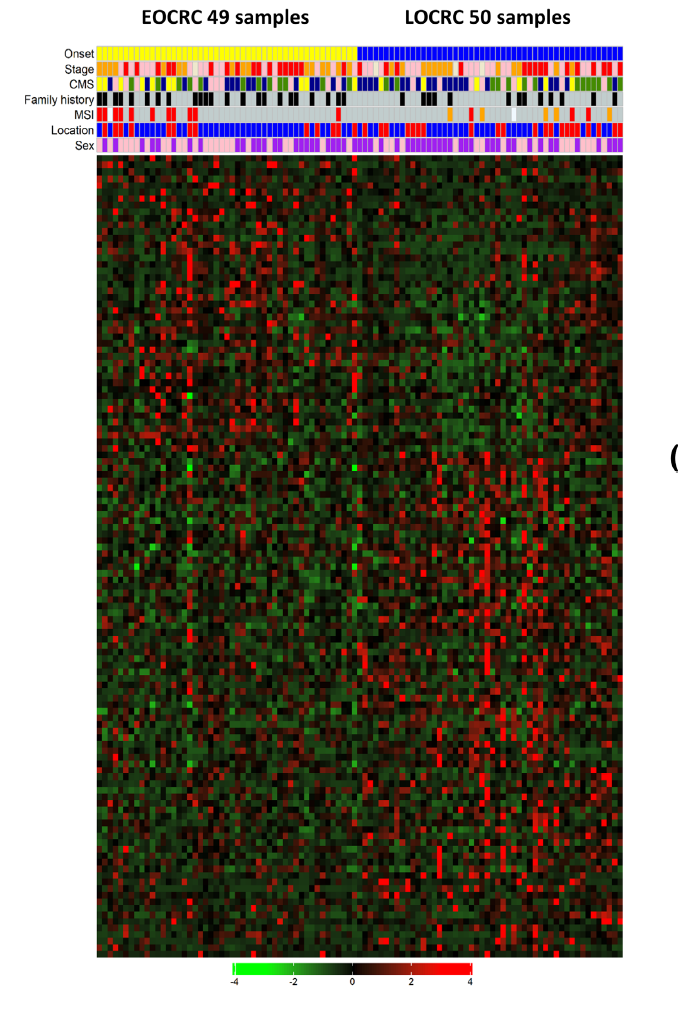
\includegraphics{./paper_heatmap.png}
\caption{sequence content}
\end{figure}

\begin{Shaded}
\begin{Highlighting}[]
\CommentTok{\# Heat map 1: based on our DEG list}
\CommentTok{\# To make a heatmap as in the paper, we need to have a matrix of z{-}scores for only the genes remaining in the filtered data}
\NormalTok{heatmap\_data }\OtherTok{\textless{}{-}} \FunctionTok{as.data.frame}\NormalTok{(}\FunctionTok{cbind}\NormalTok{(}\FunctionTok{rownames}\NormalTok{(dge\_counts\_normalized\_z\_scores), dge\_counts\_normalized\_z\_scores))}
\FunctionTok{colnames}\NormalTok{(heatmap\_data)[}\DecValTok{1}\NormalTok{] }\OtherTok{\textless{}{-}} \StringTok{"Gene"}
\NormalTok{heatmap\_data\_subset }\OtherTok{\textless{}{-}}\NormalTok{ heatmap\_data[heatmap\_data}\SpecialCharTok{$}\NormalTok{Gene }\SpecialCharTok{\%in\%}\NormalTok{ dge\_fc\_filtered}\SpecialCharTok{$}\NormalTok{genes, ] }\CommentTok{\# Get the normalized counts of the genes from the filtered and sorted DGE list }
\NormalTok{heatmap\_data\_subset }\OtherTok{\textless{}{-}}\NormalTok{ heatmap\_data\_subset[}\FunctionTok{match}\NormalTok{(dge\_fc\_filtered}\SpecialCharTok{$}\NormalTok{genes, heatmap\_data\_subset}\SpecialCharTok{$}\NormalTok{Gene), ] }\CommentTok{\# Sort as per the DGE list}
\NormalTok{heatmap\_data }\OtherTok{\textless{}{-}}\NormalTok{ heatmap\_data\_subset}
\FunctionTok{rm}\NormalTok{(heatmap\_data\_subset)}
\NormalTok{heatmap\_data }\OtherTok{\textless{}{-}} \FunctionTok{as.matrix}\NormalTok{(heatmap\_data) }\CommentTok{\#Convert to a matrix}
\NormalTok{heatmap\_data }\OtherTok{\textless{}{-}}\NormalTok{ heatmap\_data[,}\SpecialCharTok{{-}}\DecValTok{1}\NormalTok{] }\CommentTok{\#No longer need genes column for matching}
\FunctionTok{mode}\NormalTok{(heatmap\_data) }\OtherTok{\textless{}{-}}\StringTok{"numeric"}

\CommentTok{\# Generate heatmap (as per Figure 1 in the paper) using complexheatmap package (Gu, Z. Complex Heatmap Visualization. iMeta 2022.)}
\FunctionTok{library}\NormalTok{(ComplexHeatmap)}
\end{Highlighting}
\end{Shaded}

\begin{verbatim}
## Loading required package: grid
\end{verbatim}

\begin{verbatim}
## ========================================
## ComplexHeatmap version 2.14.0
## Bioconductor page: http://bioconductor.org/packages/ComplexHeatmap/
## Github page: https://github.com/jokergoo/ComplexHeatmap
## Documentation: http://jokergoo.github.io/ComplexHeatmap-reference
## 
## If you use it in published research, please cite either one:
## - Gu, Z. Complex Heatmap Visualization. iMeta 2022.
## - Gu, Z. Complex heatmaps reveal patterns and correlations in multidimensional 
##     genomic data. Bioinformatics 2016.
## 
## 
## The new InteractiveComplexHeatmap package can directly export static 
## complex heatmaps into an interactive Shiny app with zero effort. Have a try!
## 
## This message can be suppressed by:
##   suppressPackageStartupMessages(library(ComplexHeatmap))
## ========================================
\end{verbatim}

\begin{Shaded}
\begin{Highlighting}[]
\FunctionTok{library}\NormalTok{(circlize)}
\end{Highlighting}
\end{Shaded}

\begin{verbatim}
## ========================================
## circlize version 0.4.15
## CRAN page: https://cran.r-project.org/package=circlize
## Github page: https://github.com/jokergoo/circlize
## Documentation: https://jokergoo.github.io/circlize_book/book/
## 
## If you use it in published research, please cite:
## Gu, Z. circlize implements and enhances circular visualization
##   in R. Bioinformatics 2014.
## 
## This message can be suppressed by:
##   suppressPackageStartupMessages(library(circlize))
## ========================================
\end{verbatim}

\begin{Shaded}
\begin{Highlighting}[]
\NormalTok{my\_colors }\OtherTok{\textless{}{-}} \FunctionTok{colorRamp2}\NormalTok{(}\FunctionTok{c}\NormalTok{(}\SpecialCharTok{{-}}\DecValTok{4}\NormalTok{, }\DecValTok{0}\NormalTok{, }\DecValTok{4}\NormalTok{), }\FunctionTok{c}\NormalTok{(}\StringTok{"green"}\NormalTok{, }\StringTok{"black"}\NormalTok{, }\StringTok{"red"}\NormalTok{))}

\CommentTok{\#We tried to make column labels to denote whether a sample was from early or late onset group, but ran into issues with how this was displayed.}
\CommentTok{\#}
\CommentTok{\# onset\_labels = HeatmapAnnotation(onset = sample\_labels\_subset$EorL,}
\CommentTok{\#                                  col = list(onset = c("1" = "yellow", "0" = "blue")),}
\CommentTok{\#                                  gp = gpar(col = "black"), show\_legend = FALSE)}

\NormalTok{heatmap\_ourList }\OtherTok{\textless{}{-}} \FunctionTok{Heatmap}\NormalTok{(heatmap\_data, }\AttributeTok{heatmap\_legend\_param =} \FunctionTok{list}\NormalTok{(}\AttributeTok{title =} \StringTok{""}\NormalTok{), }\AttributeTok{col =}\NormalTok{ my\_colors, }
        \AttributeTok{show\_row\_dend =} \ConstantTok{FALSE}\NormalTok{, }\AttributeTok{show\_column\_dend =} \ConstantTok{FALSE}\NormalTok{,}
        \AttributeTok{row\_order =} \FunctionTok{rownames}\NormalTok{(heatmap\_data), }\AttributeTok{column\_order =}\NormalTok{ sample\_labels\_subset}\SpecialCharTok{$}\NormalTok{X}\FloatTok{.1}\NormalTok{)}

\NormalTok{heatmap\_ourList}
\end{Highlighting}
\end{Shaded}

\includegraphics{SG_LB_BMEG591E_FinalProject_files/figure-latex/unnamed-chunk-12-1.pdf}

We have left the sample names and gene names in the heatmap, so that it
can be verified that the samples are sorted into early and late-onset
groups (left half: early-onset, right half: late-onset), and the gene
list matches our gene list. It appears that in both our heatmap and the
heatmap shown in the paper, there are differences in expression between
the early- and late-onset cohorts. Both heatmaps have higher expression
levels visible in the top left and bottom right quadrants, and lower
expression in the bottom left and top right quadrants. This gives some
evidence that we correctly selected genes that were differentially
expressed between early-onset and late-onset groups. However, there are
some genes in our list with high expression across all samples that
overwhelm the signal, and there appear to be no genes with z-scores
below -2 in our heatmap. To determine whether the issue is with the list
of genes we used, we made another heatmap using the DEG list from the
authors' appendix table 1.

\begin{Shaded}
\begin{Highlighting}[]
\CommentTok{\#Second heatmap, based on authors\textquotesingle{} DEG list:}
\CommentTok{\#As before, for the heatmap input, we make a matrix of z scores, this time for only the genes in the authors\textquotesingle{} gene list}
\NormalTok{heatmap\_authorList\_data }\OtherTok{\textless{}{-}} \FunctionTok{as.data.frame}\NormalTok{(}\FunctionTok{cbind}\NormalTok{(}\FunctionTok{rownames}\NormalTok{(dge\_counts\_normalized\_z\_scores), dge\_counts\_normalized\_z\_scores))}
\FunctionTok{colnames}\NormalTok{(heatmap\_authorList\_data)[}\DecValTok{1}\NormalTok{] }\OtherTok{\textless{}{-}} \StringTok{"Gene"}
\NormalTok{heatmap\_authorList\_data\_subset }\OtherTok{\textless{}{-}}\NormalTok{ heatmap\_authorList\_data[heatmap\_authorList\_data}\SpecialCharTok{$}\NormalTok{Gene }\SpecialCharTok{\%in\%}\NormalTok{ paper\_dge\_fc}\SpecialCharTok{$}\NormalTok{Gene, ] }\CommentTok{\# Get the normalized counts of the genes from the paper\textquotesingle{}s DGE list }
\NormalTok{heatmap\_authorList\_data\_subset }\OtherTok{\textless{}{-}}\NormalTok{ heatmap\_authorList\_data\_subset[}\FunctionTok{match}\NormalTok{(paper\_dge\_fc}\SpecialCharTok{$}\NormalTok{Gene, heatmap\_authorList\_data\_subset}\SpecialCharTok{$}\NormalTok{Gene), ] }\CommentTok{\# Sort as per the DGE list}
\NormalTok{heatmap\_authorList\_data }\OtherTok{\textless{}{-}}\NormalTok{ heatmap\_authorList\_data\_subset}
\FunctionTok{rm}\NormalTok{(heatmap\_authorList\_data\_subset)}
\NormalTok{heatmap\_authorList\_data }\OtherTok{\textless{}{-}} \FunctionTok{as.matrix}\NormalTok{(heatmap\_authorList\_data) }\CommentTok{\#Convert to a matrix}
\NormalTok{heatmap\_authorList\_data }\OtherTok{\textless{}{-}}\NormalTok{ heatmap\_authorList\_data[,}\SpecialCharTok{{-}}\DecValTok{1}\NormalTok{] }\CommentTok{\#No longer need genes column for matching}
\FunctionTok{mode}\NormalTok{(heatmap\_authorList\_data) }\OtherTok{\textless{}{-}}\StringTok{"numeric"}

\CommentTok{\# For the paper\textquotesingle{}s data, generate heatmap (as per Figure 1 in the paper) using complexheatmap package (Gu, Z. Complex Heatmap Visualization. iMeta 2022.)}
\FunctionTok{library}\NormalTok{(ComplexHeatmap)}
\FunctionTok{library}\NormalTok{(circlize)}
\NormalTok{my\_colors }\OtherTok{\textless{}{-}} \FunctionTok{colorRamp2}\NormalTok{(}\FunctionTok{c}\NormalTok{(}\SpecialCharTok{{-}}\DecValTok{4}\NormalTok{, }\DecValTok{0}\NormalTok{, }\DecValTok{4}\NormalTok{), }\FunctionTok{c}\NormalTok{(}\StringTok{"green"}\NormalTok{, }\StringTok{"black"}\NormalTok{, }\StringTok{"red"}\NormalTok{))}

\NormalTok{heatmap\_authorList }\OtherTok{\textless{}{-}} \FunctionTok{Heatmap}\NormalTok{(heatmap\_authorList\_data, }\AttributeTok{heatmap\_legend\_param =} \FunctionTok{list}\NormalTok{(}\AttributeTok{title =} \StringTok{""}\NormalTok{), }\AttributeTok{col =}\NormalTok{ my\_colors, }
                     \AttributeTok{show\_row\_dend =} \ConstantTok{FALSE}\NormalTok{, }\AttributeTok{show\_column\_dend =} \ConstantTok{FALSE}\NormalTok{,}
                     \AttributeTok{row\_order =} \FunctionTok{rownames}\NormalTok{(heatmap\_authorList\_data), }\AttributeTok{column\_order =}\NormalTok{ sample\_labels\_subset}\SpecialCharTok{$}\NormalTok{X}\FloatTok{.1}\NormalTok{,}
                     \CommentTok{\#top\_annotation = onset\_labels,}
                     \AttributeTok{cluster\_columns =} \ConstantTok{FALSE}\NormalTok{)}
\NormalTok{heatmap\_authorList}
\end{Highlighting}
\end{Shaded}

\includegraphics{SG_LB_BMEG591E_FinalProject_files/figure-latex/unnamed-chunk-13-1.pdf}

This heat map also has some visible differences between the early onset
and late onset groups, but it has the same issue with globally
overexpressed genes as the first heatmap.

This suggests that the difference between our heatmap and the paper's
likely results mainly from our normalization steps, rather than our gene
list, since the gene list for the second heatmap was the same as the one
used in the paper. It is worth noting that we have sorted the samples by
cohort (early-onset and late-onset), but we do not know whether they are
sorted within each cohort in the same way as in the paper, so this could
contribute to differences in appearance between the paper's heatmap and
ours. The paper's description of the normalization method is brief (for
example, z-score normalization was not mentioned), so the order in which
steps were carried out is unclear.

Possible further approaches to replicate the paper's results might
include: - Calculating the z scores before calculating cpm, or only
calculating z scores without cpm. - Removing high-signal genes and
re-scaling (say, removing the top 6 genes with the highest sum of values
across rows). - Performing one or more of the normalization steps (TMM,
cpm, and/or z-scores) after filtering the genes. - Filtering based on
false discovery rate (FDR) instead of P-value and logFC. - Contacting
the authors to inquire about their normalization steps

In the interest of time, we will not experiment with altering the order
of these steps, but the above could be a good approach.

Part IIC: Generating a volcano plot from the DEG list

The authors made a volcano plot of -log10 P-value versus Log2FC.These
volcano plots display the genes that meet the authors' defined threshold
values for \textbar log2FC\textbar{} and -log10 P-value in the top right
and left squares.

\begin{figure}
\centering
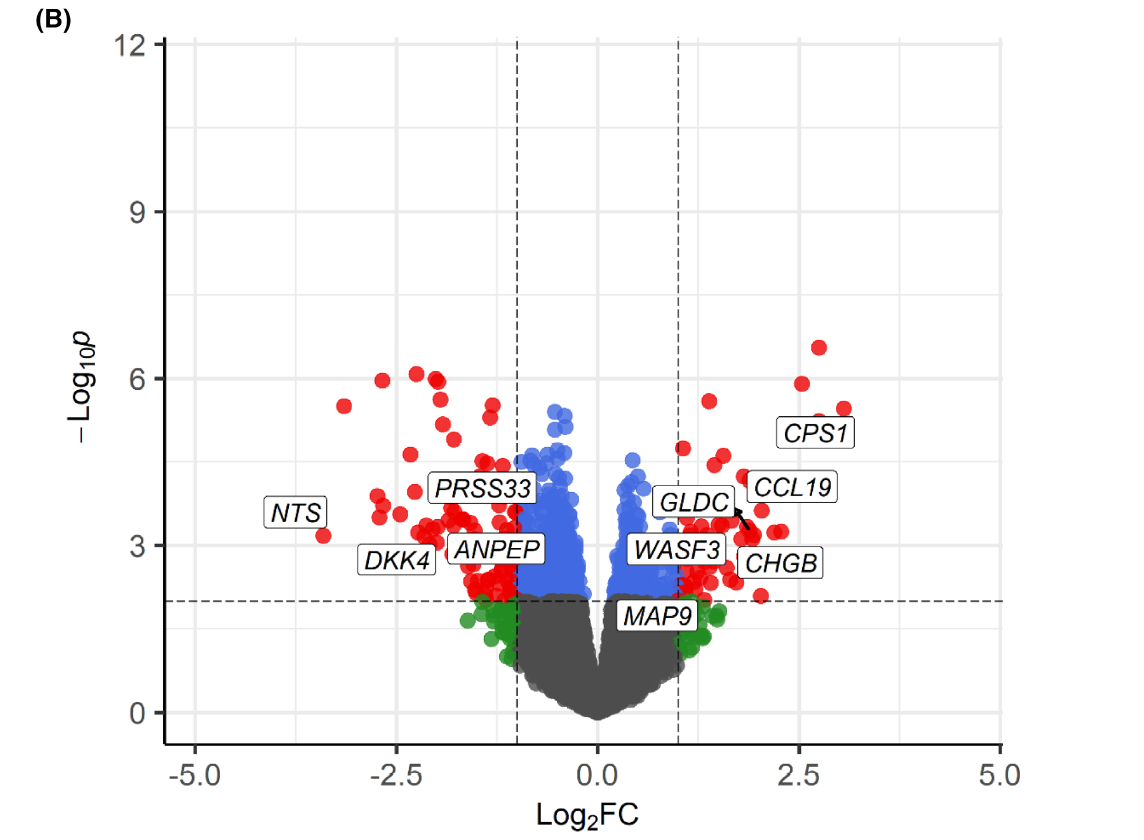
\includegraphics{./paper_volcano.png}
\caption{sequence content}
\end{figure}

\begin{Shaded}
\begin{Highlighting}[]
\CommentTok{\#Volcano plot based on our unfiltered DGE gene list:}
\FunctionTok{library}\NormalTok{(EnhancedVolcano)}
\end{Highlighting}
\end{Shaded}

\begin{verbatim}
## Loading required package: ggrepel
\end{verbatim}

\begin{Shaded}
\begin{Highlighting}[]
\NormalTok{volcano\_ourList\_unfiltered }\OtherTok{\textless{}{-}} \FunctionTok{EnhancedVolcano}\NormalTok{(dge\_fc,}
                             \AttributeTok{lab =}\NormalTok{ dge\_fc}\SpecialCharTok{$}\NormalTok{genes,}
                             \AttributeTok{x =} \StringTok{\textquotesingle{}logFC\textquotesingle{}}\NormalTok{,}
                             \AttributeTok{y =} \StringTok{\textquotesingle{}PValue\textquotesingle{}}\NormalTok{,}
                             \AttributeTok{pCutoff =} \FloatTok{0.01}\NormalTok{,}
                             \AttributeTok{FCcutoff =} \DecValTok{1}\NormalTok{,}
                             \AttributeTok{pointSize =} \FloatTok{3.0}\NormalTok{,}
                             \AttributeTok{labSize =} \FloatTok{2.0}\NormalTok{,}
                             \AttributeTok{title =} \StringTok{""}\NormalTok{,}
                             \AttributeTok{caption =} \StringTok{""}\NormalTok{)}
\NormalTok{volcano\_ourList\_unfiltered}
\end{Highlighting}
\end{Shaded}

\includegraphics{SG_LB_BMEG591E_FinalProject_files/figure-latex/unnamed-chunk-14-1.pdf}

\begin{Shaded}
\begin{Highlighting}[]
\CommentTok{\#Volcano plot based on our filtered DGE gene list:}
\FunctionTok{library}\NormalTok{(EnhancedVolcano)}
\NormalTok{volcano\_ourList\_filtered }\OtherTok{\textless{}{-}} \FunctionTok{EnhancedVolcano}\NormalTok{(dge\_fc\_filtered,}
                             \AttributeTok{lab =}\NormalTok{ dge\_fc\_filtered}\SpecialCharTok{$}\NormalTok{genes,}
                             \AttributeTok{x =} \StringTok{\textquotesingle{}logFC\textquotesingle{}}\NormalTok{,}
                             \AttributeTok{y =} \StringTok{\textquotesingle{}PValue\textquotesingle{}}\NormalTok{,}
                             \AttributeTok{pCutoff =} \FloatTok{0.01}\NormalTok{,}
                             \AttributeTok{FCcutoff =} \DecValTok{1}\NormalTok{,}
                             \AttributeTok{pointSize =} \FloatTok{3.0}\NormalTok{,}
                             \AttributeTok{labSize =} \FloatTok{2.0}\NormalTok{,}
                             \AttributeTok{title =} \StringTok{""}\NormalTok{,}
                             \AttributeTok{caption =} \StringTok{""}\NormalTok{)}
\NormalTok{volcano\_ourList\_filtered}
\end{Highlighting}
\end{Shaded}

\includegraphics{SG_LB_BMEG591E_FinalProject_files/figure-latex/unnamed-chunk-15-1.pdf}

\begin{Shaded}
\begin{Highlighting}[]
\CommentTok{\# Volcano plot based on the authors\textquotesingle{} filtered DGE gene list:}
\FunctionTok{library}\NormalTok{(EnhancedVolcano)}
\NormalTok{volcano\_authorList\_filtered }\OtherTok{\textless{}{-}} \FunctionTok{EnhancedVolcano}\NormalTok{(paper\_dge\_fc,}
                \AttributeTok{lab =}\NormalTok{ paper\_dge\_fc}\SpecialCharTok{$}\NormalTok{Gene,}
                \AttributeTok{x =} \StringTok{\textquotesingle{}logFC\textquotesingle{}}\NormalTok{,}
                \AttributeTok{y =} \StringTok{\textquotesingle{}Pvalue\textquotesingle{}}\NormalTok{,}
                \AttributeTok{pCutoff =} \FloatTok{0.01}\NormalTok{,}
                \AttributeTok{FCcutoff =} \DecValTok{1}\NormalTok{,}
                \AttributeTok{pointSize =} \FloatTok{3.0}\NormalTok{,}
                \AttributeTok{labSize =} \FloatTok{2.0}\NormalTok{,}
                \AttributeTok{title =} \StringTok{""}\NormalTok{,}
                \AttributeTok{caption =} \StringTok{""}\NormalTok{)}
\NormalTok{volcano\_authorList\_filtered}
\end{Highlighting}
\end{Shaded}

\includegraphics{SG_LB_BMEG591E_FinalProject_files/figure-latex/unnamed-chunk-16-1.pdf}

Since the filtered volcano plots only include the genes that already met
the threshold values, they only show genes in the top right and left
squares. The authors only included their filtered gene list in the
appendix, so we cannot compare their unfiltered list to ours.

Several genes appear to match in position between these four plots,
including NTS, DKK4, CCL19, and PRSS33, which gives evidence that our
replication of Figure 2 is successful. Other genes are not labelled in
the paper but appear in the same positions between the 3 plots
(e.g.~DHRS1, CCDC88B, CDK12). Our filtered volcano displays some genes
with much higher \textbar log2FC\textbar{} and -log10P values than those
identified by the authors (as discussed earlier, e.g.~the top 4 and
bottom 4 log2FC genes). It remains unclear why the authors excluded
these genes from the analysis given their low FDR values, and this bears
further investigation.

Conclusion:

Our pre-processing steps generated read counts from fastq files provided
on the GEO database. When we performed differential gene expression
analysis using the counts file provided on the GEO database, a large
number of genes matched between our filtered DEG list and the authors'
list, and the values obtained for logP, log2FC, and FDR were generally
very close. Notably, the 8 most differentially expressed genes we found
were not present in the authors' list. Since these genes also have very
low FDR values, we conclude that they bear further investigation. Our
heatmap displayed visible differences between early and late onset
colorectal cancer groups, but these differences were less obvious than
in the original paper, and we had issues with globally highly expressed
genes. Comparison with a heatmap that used the authors' DEG list led us
to conclude that the differences in our heatmap were more related to the
normalization steps than the DEG list. We proposed further steps that
could be taken to rectify our normalization. Comparison of the three
volcano plots that we generated gave good evidence that we properly
replicated the authors' methods for producing a DEG list, and further
demonstrates that the highly differentially expressed genes on our list
that were not in the authors' list warrant further investigation.
Overall, we were able to successfully repeat the steps of the authors'
analysis using the data they had made publicly available on GEO, and our
results were comparable to theirs, though there are some interesting
discrepancies that could benefit from further analysis.

Authors: Liam Brockley (26182865) and Sakshi Goyal (72365547)

Contributions: Liam and Sakshi worked together to complete the
assignment. Liam typed for the first half and Sakshi typed for the
second half.

References:

\begin{enumerate}
\def\labelenumi{\arabic{enumi}.}
\item
  Ha, Ye Jin, Yun Jae Shin, Ka Hee Tak, Jong Lyul Park, Jeong Hwan Kim,
  Jong Lyul Lee, Yong Sik Yoon, Chan Wook Kim, Seon Young Kim, and Jin
  Cheon Kim. ``Reduced Expression of Alanyl Aminopeptidase Is a Robust
  Biomarker of Non-Familial Adenomatous Polyposis and Non-Hereditary
  Nonpolyposis Colorectal Cancer Syndrome Early-Onset Colorectal
  Cancer.'' Cancer Medicine n/a, no. n/a. Accessed April 5, 2023.
  \url{https://doi.org/10.1002/cam4.5675}.
\item
  Gu, Z. Complex Heatmap Visualization. iMeta 2022.
\item
  Blighe K, Rana S, Lewis M (2022). EnhancedVolcano: Publication-ready
  volcano plots with enhanced colouring and labeling. R package version
  1.16.0, \url{https://github.com/kevinblighe/EnhancedVolcano}.
\end{enumerate}

\end{document}
